\documentclass[crop=false]{standalone}
\usepackage{standard}

\begin{document}
  \section{Beschleunigungsstrukturen, Optimierung und weitere Features} % (fold)
  \label{sec:beschleunigungsstrukturen_optimierung_und_weitere_features}
    Auf den in Abschnitt \ref{sec:basics} beschriebenen Grundlagen bauten alle weiteren Optimierungen und Features auf.
    Ich habe mich mit diesem Projekt innerhalb meiner Arbeitsgruppe seit über vier Jahren beschäftigt und folglich einige Verbesserungen vorgenommen, sowie Messungen durchgeführt und Erfahrungen gesammelt.
    Die genaue Beschreibung der Lösungsmethoden und Ergebnisse aller Veränderungen würde über den Rahmen dieses Berichts hinausgehen.
    Demzufolge sind im Folgenden viele der Features und Optimierungen in einer kürzeren Form dargestellt.
    So ist es mir möglich, eine verständliche Zusammenfassung der Arbeit am Projekt zu vermitteln.

    \subsection{Linear Bounding Volume Hierarchies} % (fold)
    \label{sub:linear_bounding_volume_hierarchies}
      Beschleunigungsstrukturen stellen eines der Kernelemente eines jeden Raytracers dar und funktionieren unabhängig von der Hardware.
      Ohne Algorithmen, die die Anzahl der Schnittpunkttests für jeden Strahl reduzieren, wäre die Zeit einen einzelnen Strahl durch die Szene zu schießen proportional zur Anzahl der Dreiecke.
      In den meisten Fällen handelt es sich hierbei jedoch um Zeitverschwendung, da ein Strahl die überwiegende Mehrheit der Dreiecke gar nicht schneidet.
      Das Ziel von Beschleunigungsstrukturen besteht darin, Gruppen von nicht-schneidenden Dreiecken schnell zu verwerfen und die Übrigen zu sortieren, um nahegelegene Dreiecke zu bevorzugen.

      \textit{Bounding Volume Hierachies} (BVH) sind Beschleunigungsstrukturen.
      Sie unterteilen eine gegebene Szene in eine Hierarchie von disjunkten Mengen von Dreiecken.
      Abbildung \ref{fig:bvh-scheme} zeigt diese Methode anhand zweier Skizzen.
      Dreiecke werden in den Blättern der Hierarchie gespeichert, während sogenannte \textit{Bounding Boxes} die Knoten zwischen den Blättern füllen.
      Ein Strahl traversiert den Baum indem in jedem Knoten, an welchem er vorbeikommt, einen Schnittpunkttest mit der \textit{Bounding Box} durchführt.
      Fällt der Test negativ aus, so wird der Knoten mit seinen Kindern verworfen.
      \begin{figure}[h]
        \center
        \begin{subfigure}[b]{0.49\textwidth}
          \center
          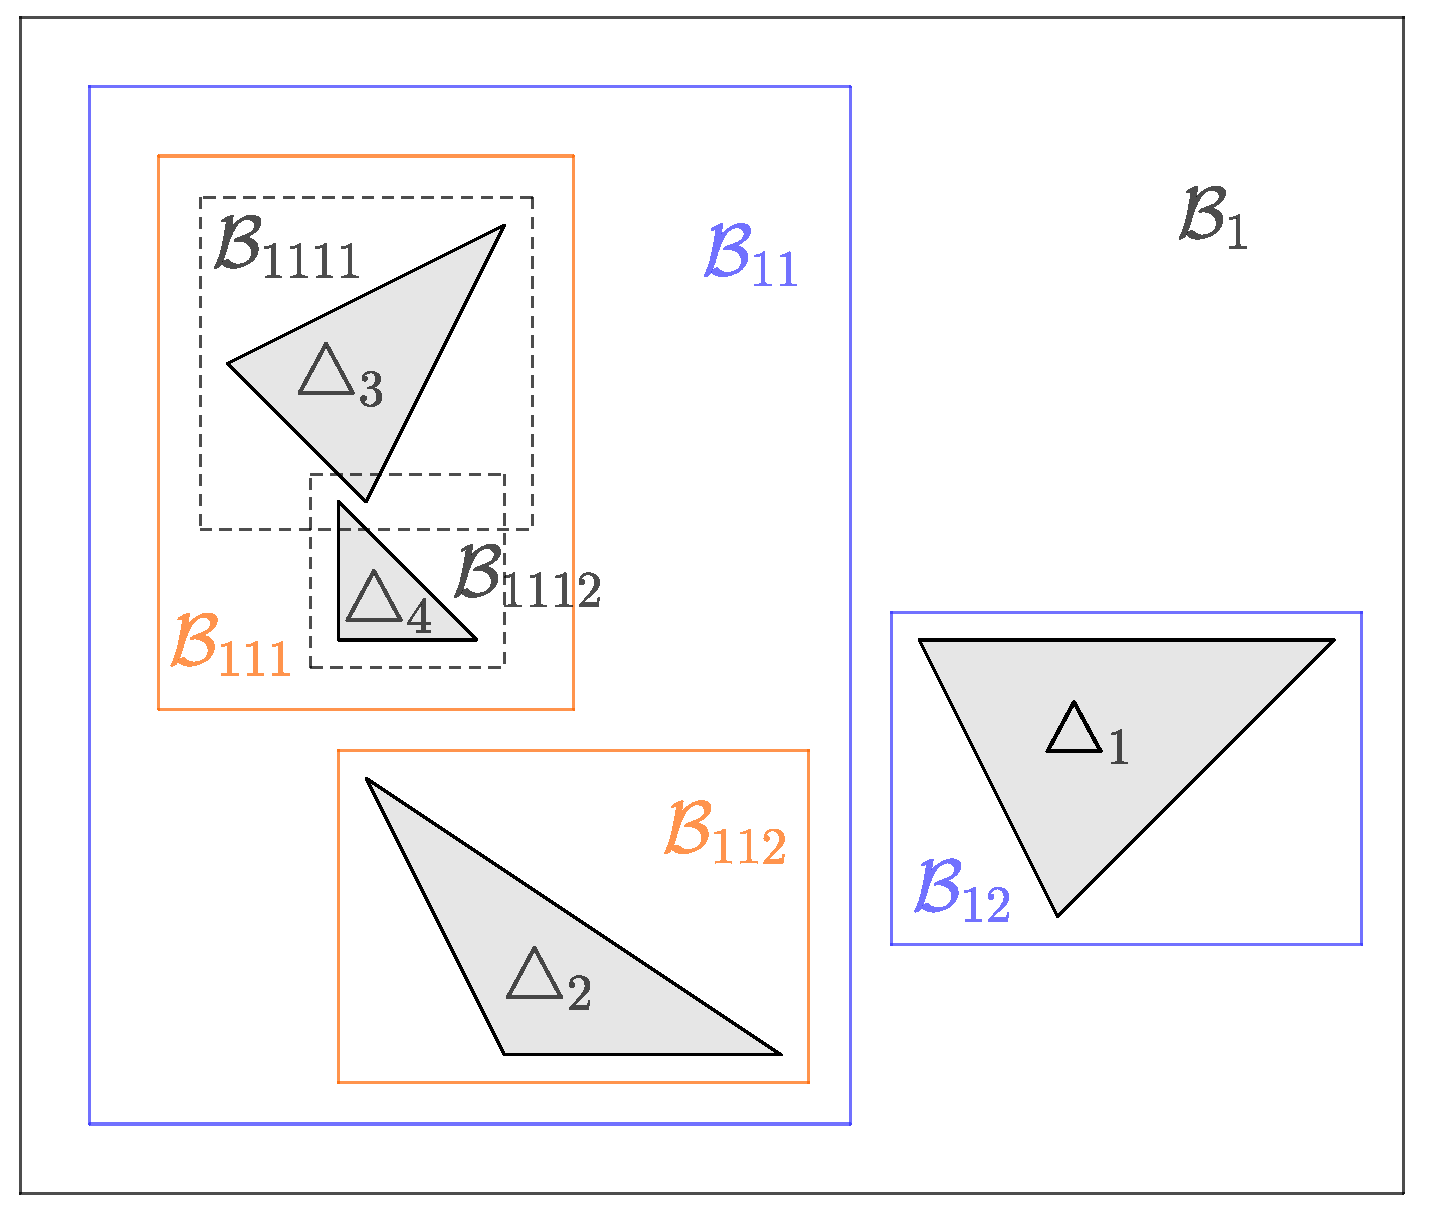
\includegraphics[width=0.95\textwidth]{images/bvh_bounding_boxes.pdf}
        \end{subfigure}
        \begin{subfigure}[b]{0.49\textwidth}
          \center
          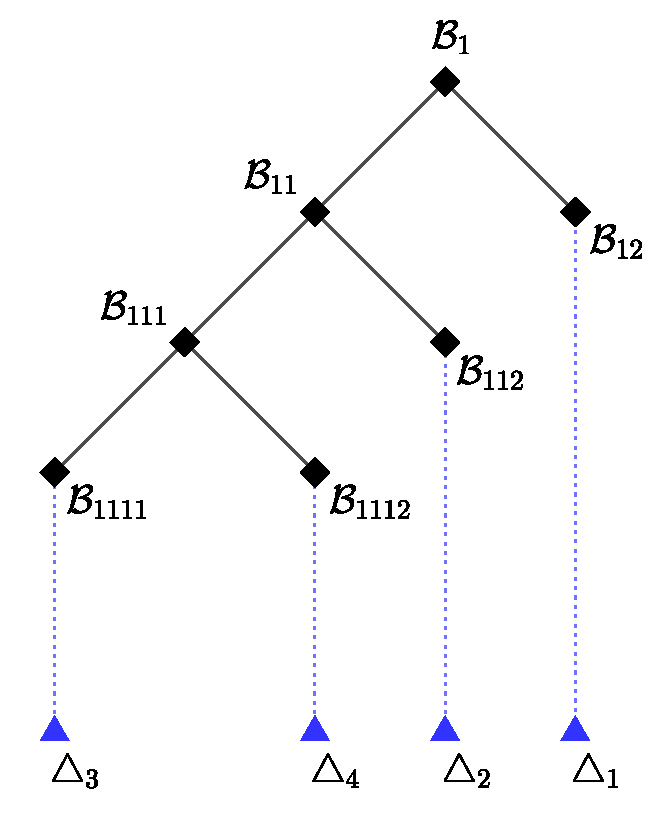
\includegraphics[width=0.75\textwidth]{images/bvh_tree.pdf}
        \end{subfigure}
        \caption{%
          Die Abbildungen zeigen die skizzenhafte Darstellung einer möglichen BVH einer Szene bestehend aus den Dreiecken $\triangle_1$, $\triangle_2$, $\triangle_3$ und $\triangle_4$.
          Im linken Bild sind die \textit{Bounding Boxes} der BVH und im rechten Bild deren zugehörige Verknüpfungen im Sinne eines Baums gezeigt.
        }
        \label{fig:bvh-scheme}
      \end{figure}

      Um die Schnittpunktberechnung zwischen Strahl und \textit{Bounding Box} so weit wie möglich zu vereinfachen, werden an den Koordinatenachsen ausgerichtete \textit{Bounding Boxes} (AABB, engl.: \textit{axis-aligned bounding box}) verwendet.
      Diese lassen sich eindeutig durch die Angabe zweier ihrer gegenüberliegenden Eckpunkte beschreiben.
      Eine AABB beschreibt damit einen Quader im Raum.
      Aus diesem Grund muss für jede der sechs Flächen ein Schnittpunkttest durchgeführt werden.
      Durch die Ausrichtung an den Koordinatenachsen vereinfachen sich diese sechs Tests jedoch zu einer Division, sechs Additionen und sechs Multiplikationen.

      Um BVHs zu konstruieren lassen sich diverse Algorithmen verwenden.
      Im Projekt wählte ich eine Methode, die sowohl auf der CPU als auch GPU effizient funktionieren sollte.
      \textit{Linear Bounding Volume Hierarchies} (LBVH) können in linearer Zeit bezüglich der Anzahl der Dreiecke konstruiert werden.
      Sie sind vergleichsweise einfach parallelisierbar und skalieren sowohl auf der CPU als auch auf der GPU.

      Die Idee besteht darin, die Konstruktion einer LBVH auf ein Sortierverfahren zurückzuführen.
      Da es im dreidimensionalem Raum keine eindeutig ausgezeichnete Ordnung gibt, verwendet man \textit{Morton Codes}.
      Diese bilden naheliegende dreidimensionale Punkte auf naheliegende eindimensionale Punkte entlang einer Kurve ab.
      Aufgrund ihrer charakteristischen Form wird diese Kurve auch die Z-Kurve genannt.
      Abbildung \ref{fig:morton-curve-scheme} zeigt den Verlauf der Morton-Kurve für zwei unterschiedlich feine Gitter.
      Zudem zeigt sie, dass \textit{Morton Codes} auf einer simplen Transformation basieren.
      Gegeben sei für ein $n\in\setNatural$ ein Tupel natürlicher Zahlen $k\in\setNatural_0^n$.
      Die Binärdarstellung einer Koordinate $k_i$ für $i\in\setNatural_0$ mit $i<n$ sei gegeben durch
      \[
        k_i = (\cdots k_{i3}\, k_{i2}\, k_{i1}\, k_{i0})_2
      \]
      In diesem Falle berechnet sich der \textit{Morton Code} $m(k)$ von $k$ durch den folgenden Ausdruck.
      \[
        m(k) \define (\cdots k_{22}\, k_{12}\, k_{02}\cdots k_{21}\, k_{11}\, k_{01}\cdots k_{20}\,k_{10}\,k_{00})_2
      \]
      Durch die Verwendung von \textit{Radix Sort} und der \textit{Morton Codes} der Dreiecksmittelpunkte lässt sich nun durch ein \textit{Bottom-Up}-Verfahren die BVH effizient und parallel konstruieren.
      \begin{figure}[h]
        \center
        \begin{subfigure}[c]{0.49\textwidth}
          \center
          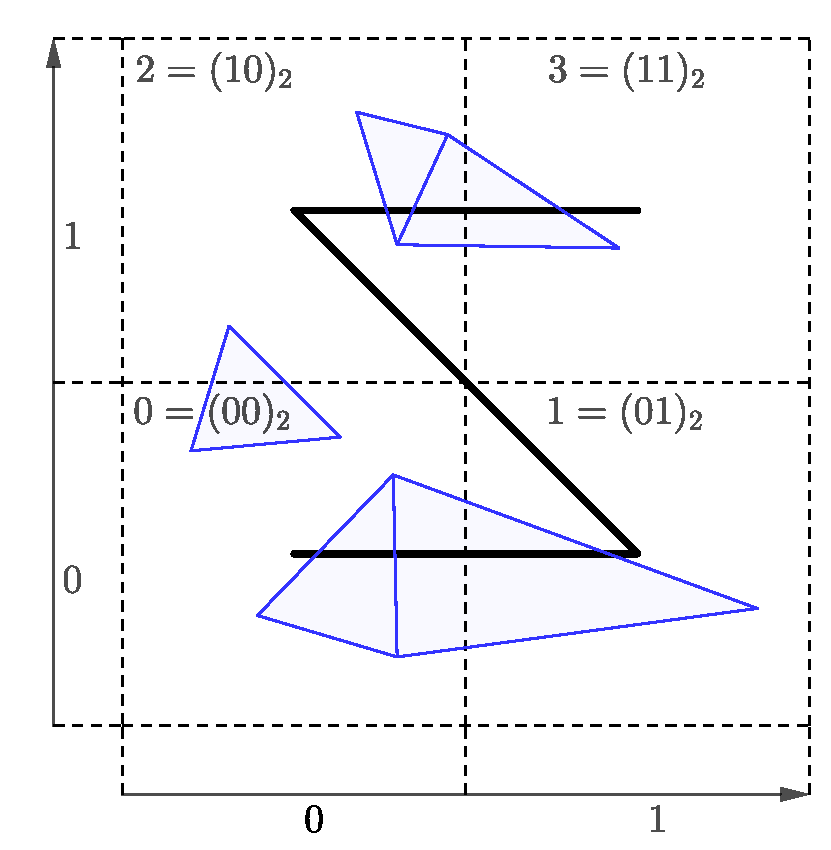
\includegraphics[width=0.95\textwidth]{images/morton_curve_1.pdf}
        \end{subfigure}
        \begin{subfigure}[c]{0.478\textwidth}
          \center
          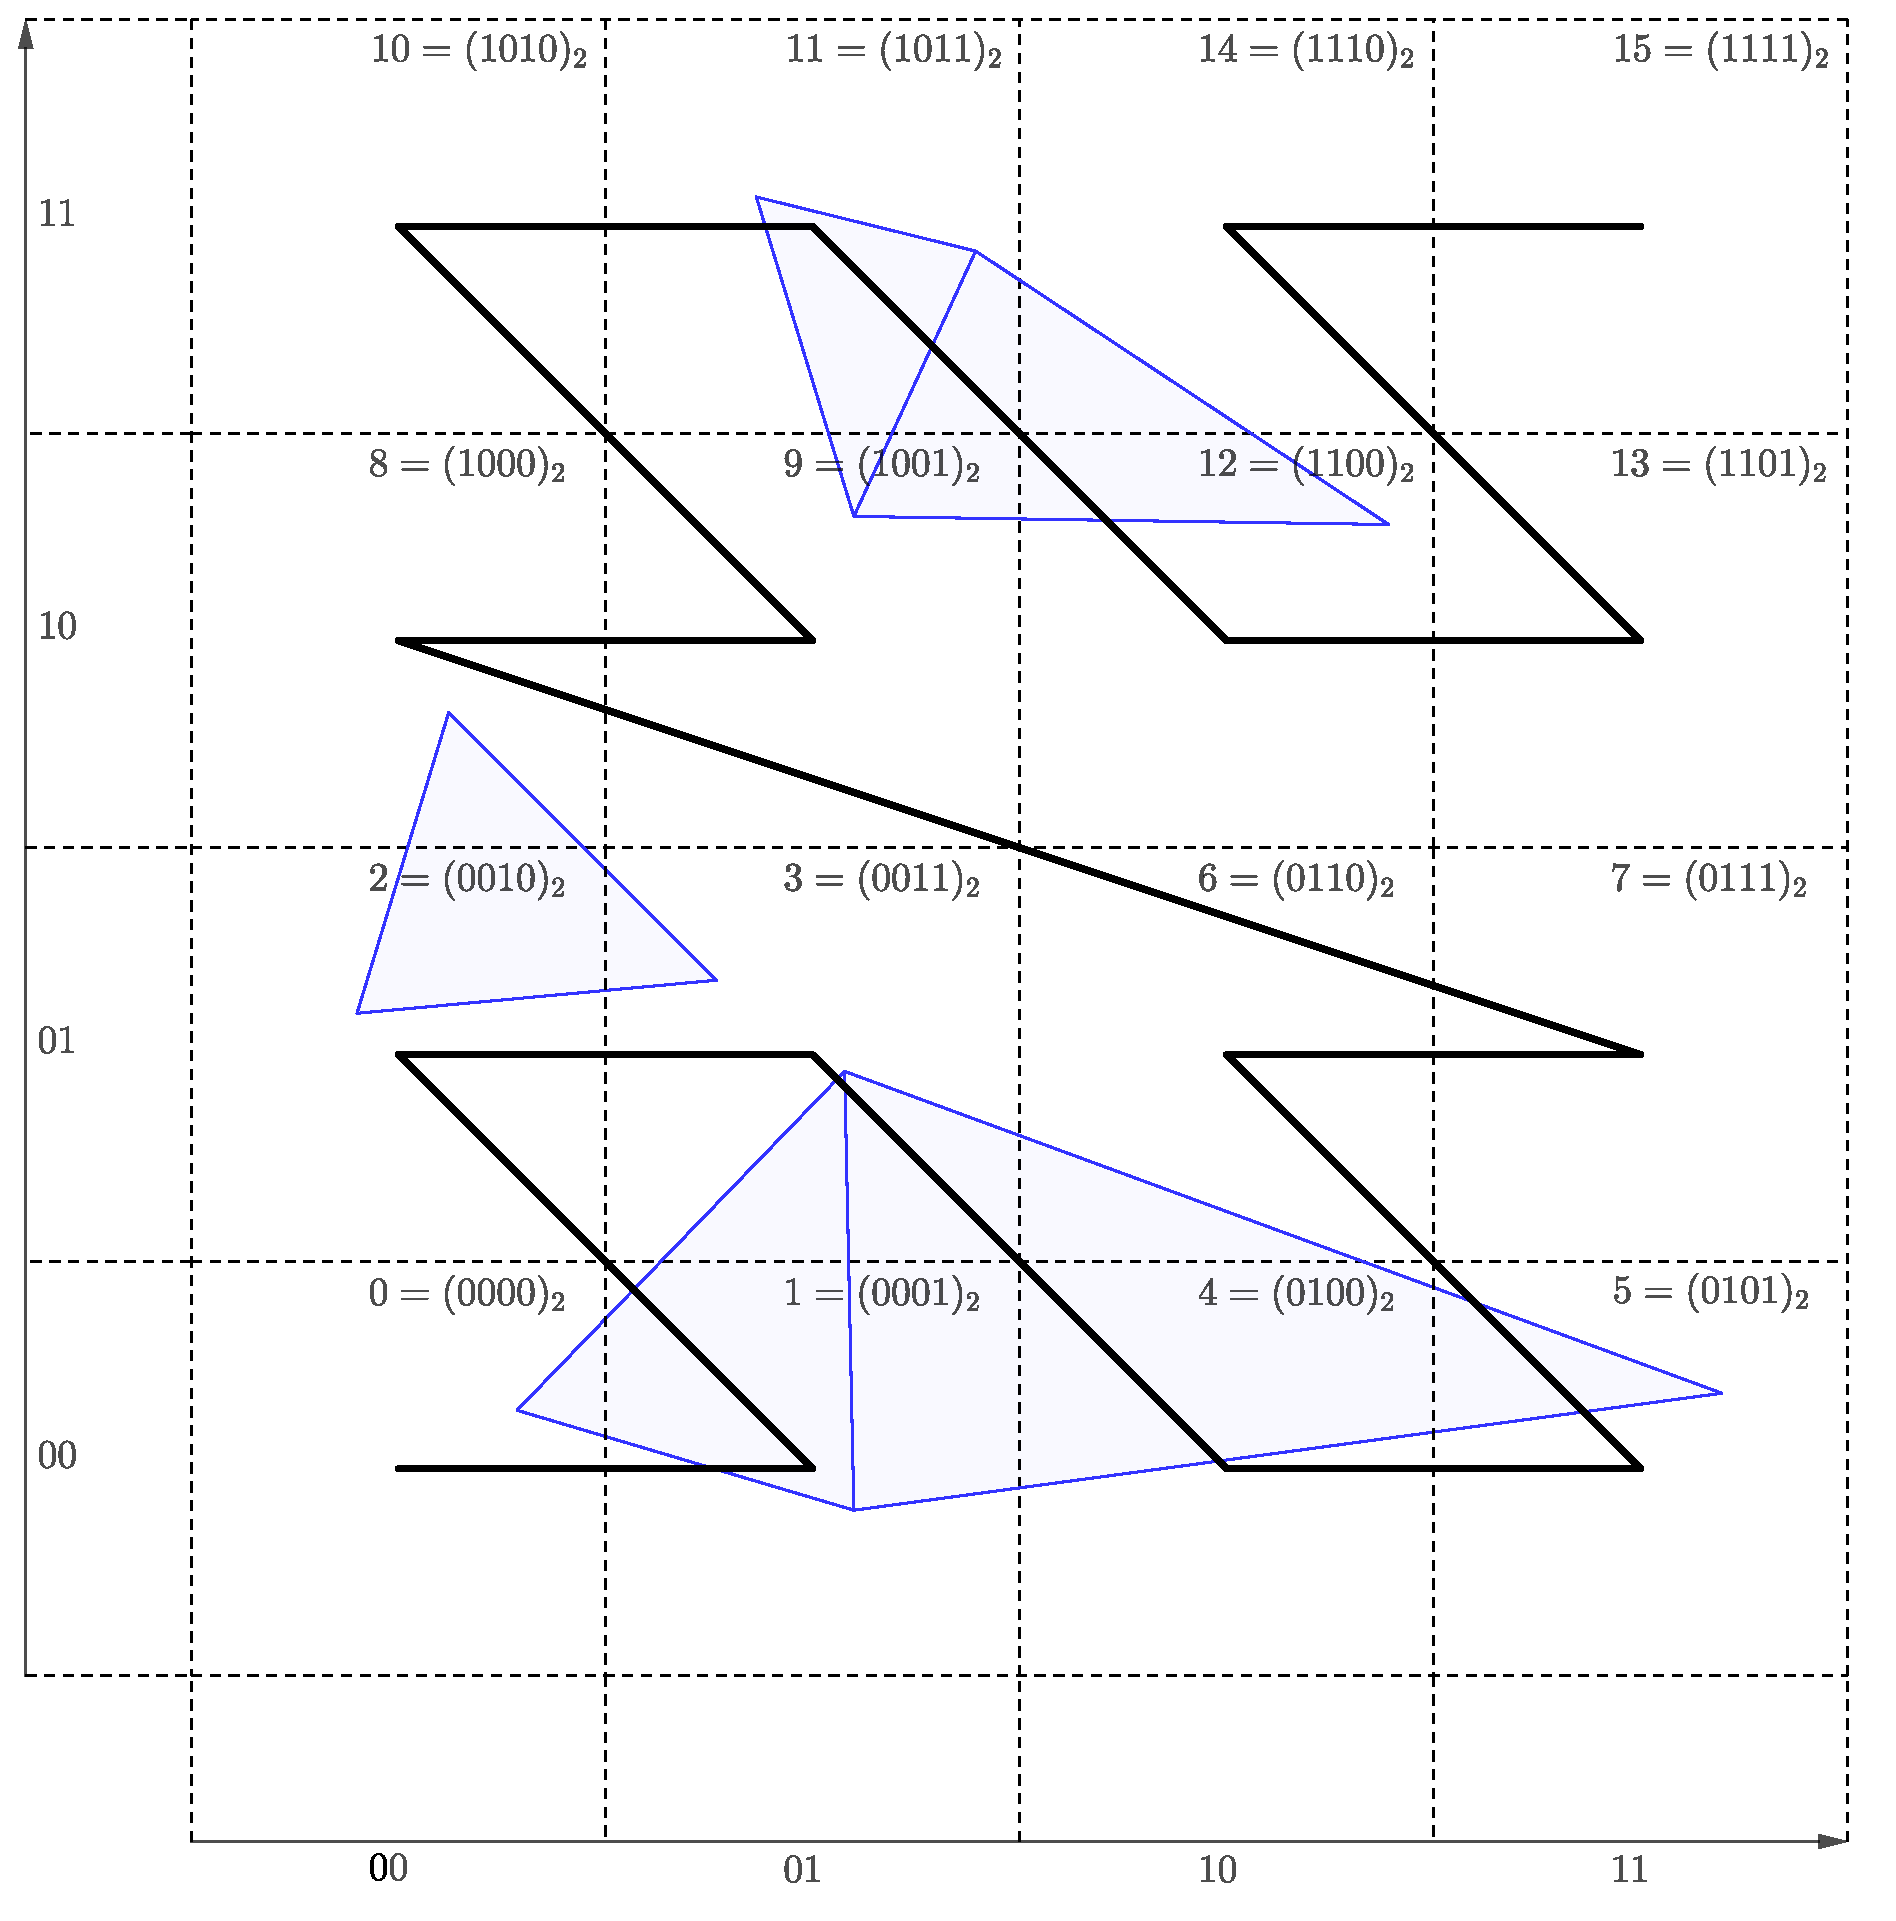
\includegraphics[width=0.95\textwidth]{images/morton_curve_2.pdf}
        \end{subfigure}
        \caption{%
          Die Abbildung zeigt den Verlauf der Morton-Kurve durch die Szene für zwei unterschiedliche Verfeinerungsgrade der Gitter.
        }
        \label{fig:morton-curve-scheme}
      \end{figure}

      Die Struktur einer BVH führt dazu, dass die Laufzeitkomplexität im Durchschnitt logarithmisch statt linear in der Anzahl der Dreiecke verläuft.
      Dies führte zu einer dramatischen Verbesserung der vorherigen Ergebnisse.
      Abbildung \ref{fig:lbvh-results} zeigt vier der im Projekt verwendeten hochkomplexen Modelle.
      Jede Szene konnte durch User-Interaktion mit durchschnittlich $50\appendUnit{FPS}$ rotiert werden.
      Damit übertraf die Verwendung der LBVH jede meiner Erwartungen.
      Auch die Konstruktion der LBVH war innerhalb von ein paar Millisekunden abgeschlossen.
      Doch auch dieser extrem performante Build-Prozess offenbarte nach genaueren Messungen einige Schwachstellen.
      Die entstehende BVH stellt keine optimale BVH der Szene dar.
      Sobald sich die Kamera innerhalb eines Objektes befand, verlangsamte sich das gesamte Rendering.
      Im Verlauf des Projektes wurden innerhalb meiner Arbeitsgruppe weitere Verfahren zur Konstruktion von BVHs eingebaut.
      Es scheint als würden die besten Bäume durch hybride Verwendung von mehreren Methoden entstehen.
      \begin{figure}[h]
        \center
        \begin{subfigure}[b]{0.24\textwidth}
          \center
          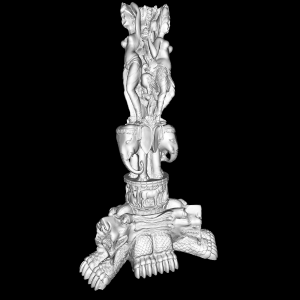
\includegraphics[width=0.95\textwidth]{images/thai_statue.png}
          \caption{\textit{Thai Statue}}
        \end{subfigure}
        \begin{subfigure}[b]{0.24\textwidth}
          \center
          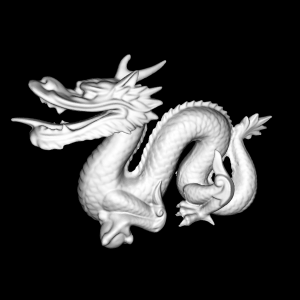
\includegraphics[width=0.95\textwidth]{images/dragon.png}
          \caption{\textit{Chinese Dragon}}
        \end{subfigure}
        \begin{subfigure}[b]{0.24\textwidth}
          \center
          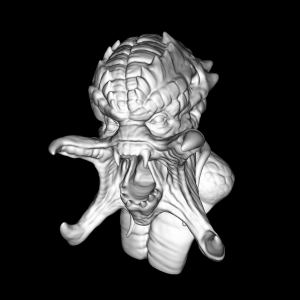
\includegraphics[width=0.95\textwidth]{images/predator.png}
          \caption{\textit{Predator}}
        \end{subfigure}
        \begin{subfigure}[b]{0.24\textwidth}
          \center
          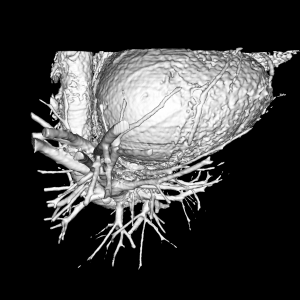
\includegraphics[width=0.95\textwidth]{images/half_heart.png}
          \caption{\textit{Half Heart}}
        \end{subfigure}
        \caption{%
          Die Abbildungen zeigen vier Modell, welche durch den Raytracer gerendert wurden.
          Aufgrund der extrem hohen Dreiecksanzahl war es erst durch die Verwendung einer Beschleunigungsstruktur, wie der LBVH, möglich diese Bilder in Echtzeit zu generieren.
        }
        \label{fig:lbvh-results}
      \end{figure}

    % subsection linear_bounding_volume_hierarchies (end)

    \subsection{Path Tracing} % (fold)
    \label{sub:path_tracing}
      Da der Raytracer vor allem der Visualisierung dienen sollte, war es nötig den Lichttransport innerhalb einer Szene zu simulieren.
      In der Theorie wird die Simulation von Lichtverteilungen durch die Rendergleichung (engl.: \textit{rendering equation} oder \textit{light transport equation}) beschrieben.
      Dabei handelt es sich um eine Fredholm-Integralgleichung 2.~Art für die Strahldichte der gesamten Szene.
      Sie kann mithilfe der Energieerhaltung und Theoremen der geometrischen Optik und Radiometrie hergeleitet werden.
      Im Allgemeinen besitzt dieses Gleichung keine geschlossene Lösung.
      Ihre Verwendung bedingt zudem die Implementierung von physikalischen Materialien, die Licht reflektieren, absorbieren und brechen.
      Die Materialien beschreiben dabei die genaue Interaktion von Lichtstrahlen mit den Oberflächen von Objekten durch bidirektionale Streuungsverteilungsfunktionen (BSDF, engl.: \textit{bidirectional scattering distribution function}).

      Eine BSDF gibt an, welcher Anteil des einfallenden Lichtes bezüglich der Einfallsrichtung in eine bestimmte Richtung gestreut wird.
      Sie stellt damit eine Verallgemeinerung der idealen Reflexion und Brechung an Oberflächen dar.
      Die Konstruktion komplexer Materialien erfolgte zumeist durch Bildung einer Linearkombination bereits bekannter und gut beschreibbarer BSDFs, wie der Lambertsch diffuse Strahler oder die \textit{Glossy Reflection}, sodass diese effizient durch die Speicherung von Koeffizienten implementiert werden konnten.

      Für die numerische Lösung der Rendergleichung transformiert man diese in ihre Pfadintegral-Formulierung.
      Die Integrale lassen sich nun durch Monte-Carlo Methoden erwartungstreu schätzen.
      Trifft ein Primärstrahl auf die Oberfläche, so wird durch die randomisierte \textit{Russian Roulette}-Methode entschieden, ob dieser Strahl reflektiert, absorbiert oder transmittiert wird.
      Auf der Basis dieser Entscheidung wird eine neuer zufälliger Strahl auf der entsprechenden Hemisphäre generiert, der wiederum den kompletten \textit{Path Tracing}-Prozess durchläuft.
      Um die Farbe eines Pixels mit einem geringen Fehler zu schätzen, ist es notwendig eine große Anzahl dieser Pfade auszuwerten.

      Abbildung \ref{fig:path-tracing-results} zeigt diverse durch \textit{Path Tracing} generierte Bilder.
      Je nach Beleuchtung und Aufbau einer Szene konvergiert der Algorithmus unterschiedlich schnell.
      Vor allem im Inneren von Objekten muss eine enorm lange Zeit vergehen, bis ein akzeptables Ergebnis zu sehen ist.
      Es konnte leider nicht gemessen werden, ob die simulierten Ergebnisse auch der Wirklichkeit entsprachen.
      Dennoch schienen die Bilder für das menschliche Auge durchaus realistische und nicht Computer generiert.
      \begin{figure}[h]
        \center
        \begin{subfigure}[b]{0.614\textwidth}
          \center
          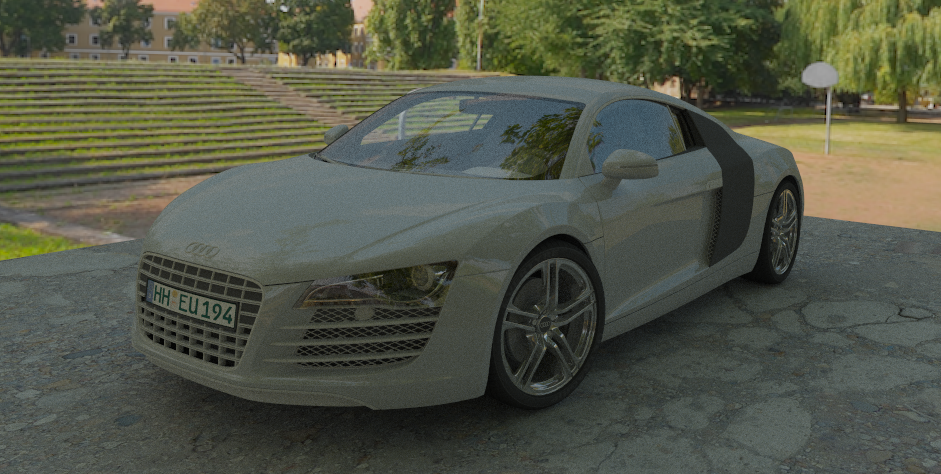
\includegraphics[width=0.95\textwidth]{images/path_tracing-audi_r8.png}
          \caption{\textit{Audi R8}}
        \end{subfigure}
        \begin{subfigure}[b]{0.38\textwidth}
          \center
          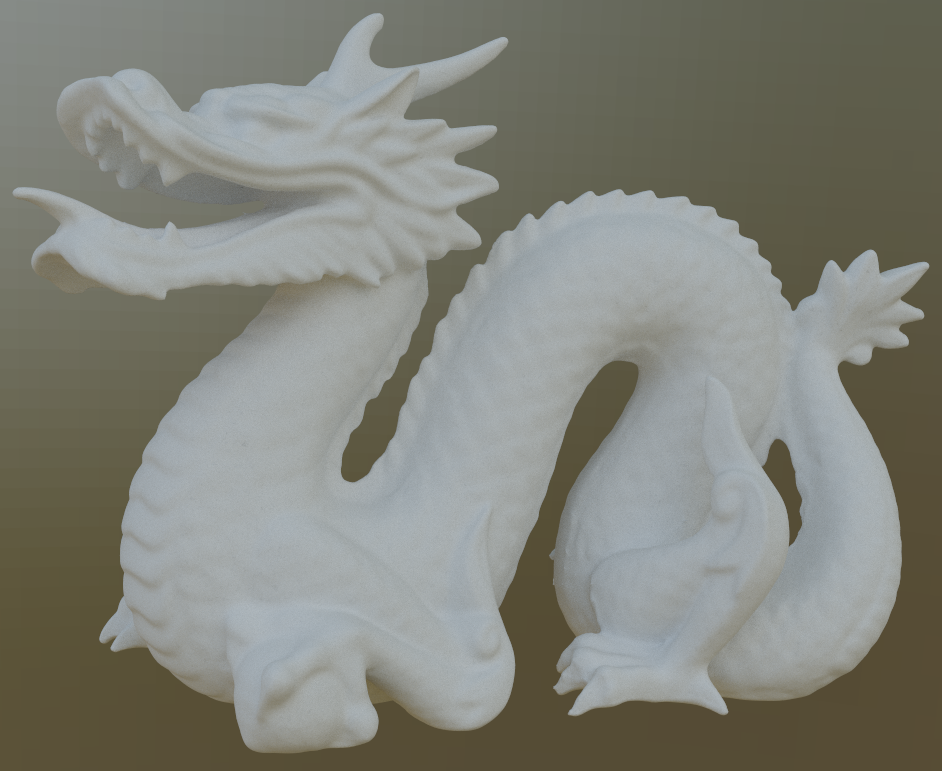
\includegraphics[width=0.95\textwidth]{images/path_tracing-dragon.png}
          \caption{\textit{Chinese Dragon}}
        \end{subfigure}

        \begin{subfigure}[b]{0.635\textwidth}
          \center
          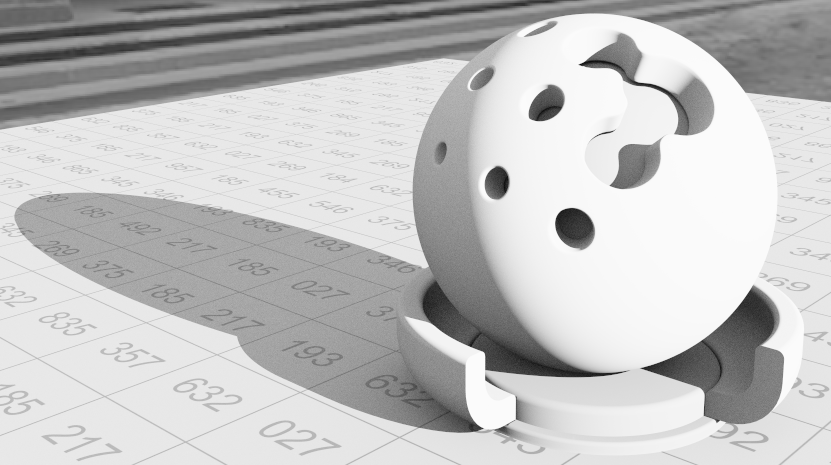
\includegraphics[width=0.95\textwidth]{images/path_tracing-shaderball.png}
          \caption{\textit{Shaderball}}
        \end{subfigure}
        \begin{subfigure}[b]{0.358\textwidth}
          \center
          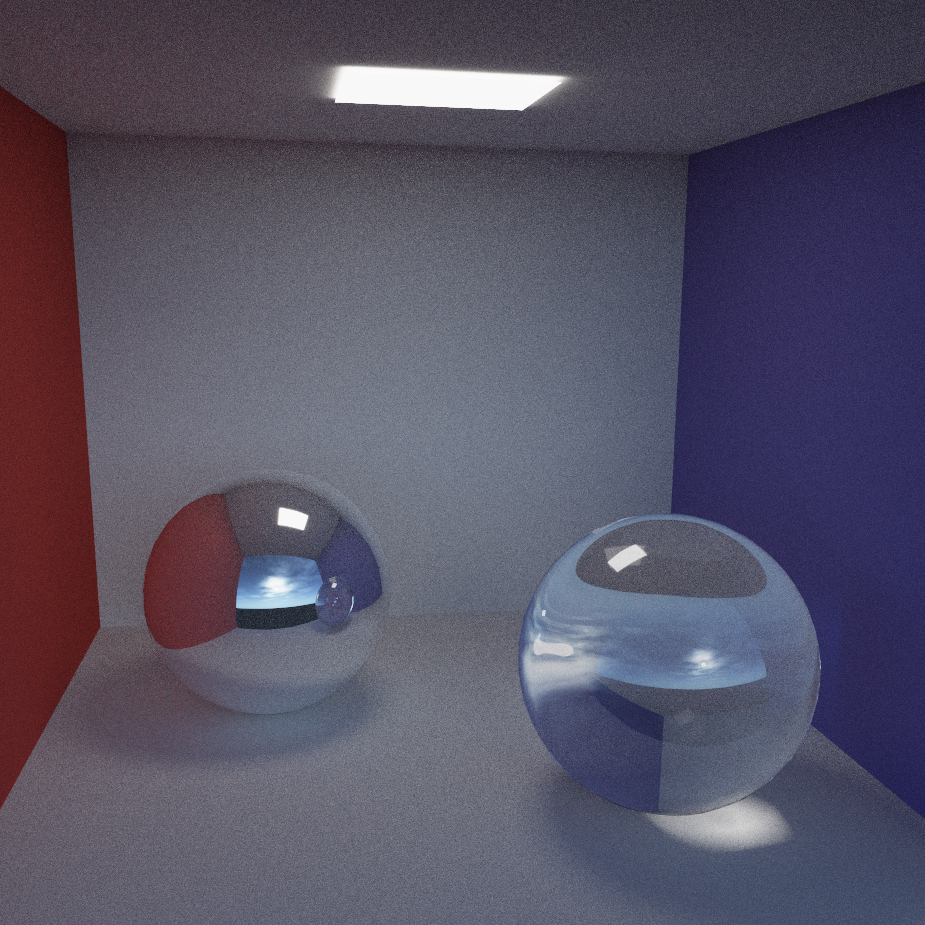
\includegraphics[width=0.95\textwidth]{images/path_tracing-cornell_box.png}
          \caption{\textit{Cornell Box}}
        \end{subfigure}
        \caption{%
          Die Abbildungen wurden mithilfe des hier implementierten \textit{Path Tracing}-Verfahrens für verschiedene Modelle erzeugt.
          Die Materialien der Modelle wurden durch ideale Reflexionen, Brechungen und Lambertsche Strahler beschrieben.
          Für jeden Pixel wurden 1024 zufällige Pfade ausgewertet.
        }
        \label{fig:path-tracing-results}
      \end{figure}
    % subsection path_tracing (end)

    \subsection{Optimierungen auf der CPU} % (fold)
    \label{sub:optimierungen_auf_cpu}
      Neben Features und Beschleunigungsstrukturen gab es auch Hardware-basierte Verfahren zur Optimierung des Quellcodes.
      Innerhalb der Arbeitsgruppe habe ich mich mit \textit{Cache Coherency} und der Parallelisierung auseinandergesetzt.
      Grundsätzlich gibt es mehrere Formen der Parallelisierung.
      Für das Projekt beschäftigte ich mich vor allem mit SIMD (engl.: \textit{single input multiple data}) und MIMD (engl.: \textit{multiple input multiple data}) beziehungsweise \textit{Thread-Level-Parallelism}.
      Begründet war dies durch die Tatsache das der Compiler bereits automatisch einen großen Teil des Quelltexts effizient optimierte.

      Durch die Funktionsweise des Rendering-Verfahrens stellte die Implementierung von Thread-Parallelismus kein Problem dar.
      Für jeden Pixel des Pixelpuffers mussten mehrere hundert Strahlen durch \textit{Path Tracing} unabhängig voneinander ausgewertet werden.
      Gerade die Unabhängigkeit der verschiedenen Pixel ermöglichte es mir, den Pixelpuffer in mehrere Pixelblöcke einzuteilen und diese dann den Threads des Computers zuzuweisen.
      Da unterschiedliche Pixelblöcke je nach Szene und Beleuchtung auch unterschiedlich lange berechnet wurden, verwendete ich eine dynamische Zuweisung der Pixelblöcke zu den Threads (siehe \textit{load balancing}).
      Dieses Verfahren wurde sowohl durch \textit{OpenMP} als auch durch eine vom ITWM entwickelte Thread-Bibliothek \textit{MCTP} umgesetzt.

      Die Ergebnisse dieser Implementierung entsprachen voll und ganz den Erwartungen.
      Die Geschwindigkeit der Bildgenerierung konnte um die Anzahl der Cores der CPU eines Computers vervielfacht werden.

      Die manuelle Parallelisierung durch SIMD ist prinzipiell nur durch spezielle Bibliotheken, wie \textit{OpenMP}, oder durch das Einbinden der sogenannten \textit{Intrinsics}, wie den \textit{Streaming SIMD Extensions} (SSE) oder den \textit{Advanced Vector Extensions} (AVX),  möglich.
      Sie erlauben es dem Entwickler im Quelltext auf die Vektorregister der CPU zuzugreifen.
      Je nach Baujahr eines Computers passen in diese Register vier bis sechzehn Gleitkommazahlen einfacher Genauigkeit hinein.
      Demnach bedeutet eine effiziente Nutzung dieser Register eine vier- bis sechzehnfache Steigerung der Performance.
      Die manuelle Verwendung dieser \textit{Intrinsics} geht jedoch mit einer starken Hardwarebindung einher.
      Code der durch AVX optimiert wurde, lässt sich nur auf Computern, die ebenfalls AVX kennen, ausführen.
      Aus diesem Grund werden häufig mehrere Varianten eines Algorithmus implementiert, um eine maximale Portabilität zu erreichen.

      Im Projekt konzentrierte ich mich auf den Kernel des Raytracers.
      Jeder Strahl muss die BVH traversieren um einen Schnittpunkt zu ermitteln.
      Anstatt innerhalb eines Threads die Strahlen sequentiell zu testen, kann man dazu übergehen, mehrere Strahlen in einem Strahlenpaket durch mehrere Vektorregister zu speichern.
      Diese Neustrukturierung geht davon aus, dass alle Strahlen, die in diesem Paket vorkommen, kohärent sind, beziehungsweise einen ähnlichen Strahlenverlauf aufweisen.
      Diese Annahme ist zumindest für Primärstrahlen, die von der Kamera ausgesendet werden, bis zu einem gewissen Grade erfüllt.
      Bei der eigentlichen Traversierung wird das Strahlenpaket wie ein einziger Strahl behandelt und auf Schnittpunkte mit den einzelnen AABB der Knoten getestet.
      Ein Knoten und dessen Kinder werden jedoch nur verworfen, falls keiner der Strahlen im Paket die zugehörige AABB schneidet.
      Sind die Strahlen, wie vorher angenommen, kohärent, so lassen sich die Schnittpunkte der Strahlen eines Pakets genauso so schnell wie der Schnittpunkt eines einzelnen Strahls berechnen.
      Sollten die Strahlen allerdings eine starke Divergenz aufweisen, so wird die Effizienz des Verfahrens reduziert, da mehr Äste der BVH traversiert werden müssen.

      Die Ergebnisse dieser Implementierung zeigten eine drei- bis fünfzehnfache Steigerung der Performance für die Berechnung von Primärstrahlen.
      Sekundärstrahlen, welche zum Beispiele durch die Reflexion an Oberflächen entstehen, ließen die \textit{Frame Rate} einbrechen.
      In extremen Fällen konnte sogar festgestellt werden, dass die automatische Optimierung des Compilers bessere Ergebnisse lieferte.
    % subsection optimierungen_auf_cpu (end)
  % section beschleunigungsstrukturen_optimierung_und_weitere_features (end)
\end{document}